\newpage

\ifthenelse{\boolean{website_upload}}{
	\phantomsection
    \includepdf{docs/appendix_graphics.pdf}

	\addtocounter{appendixNum}{1}
	\addcontentsline{toc}{section}{ПРИЛОЖЕНИЕ \Asbuk{appendixNum}.~Копии листов графической части}
	\setcounter{figure}{0}
	\renewcommand{\thefigure}{\Asbuk{appendixNum}\arabic{figure}}
}{
    \begin{center}
      \myAppendix{Копии листов графической части.}
    \end{center}

    \begin{enumerate}
      \item Структурная схема системы;
      \item Схема электрическая принципиальная аппаратной части системы;
      \item Граф состояний интерфейса;
      \item Формы интерфейса;
      \item Диаграммы классов программного обеспечения;
      \item Схемы алгоритмов модулей (подпрограмм).
    \end{enumerate}
}

{
\setcounter{figure}{0}
\renewcommand{\thefigure}{\Asbuk{appendixNum}\arabic{figure}}

\newpage
\begin{figure}[H]
    \centering
    \fbox{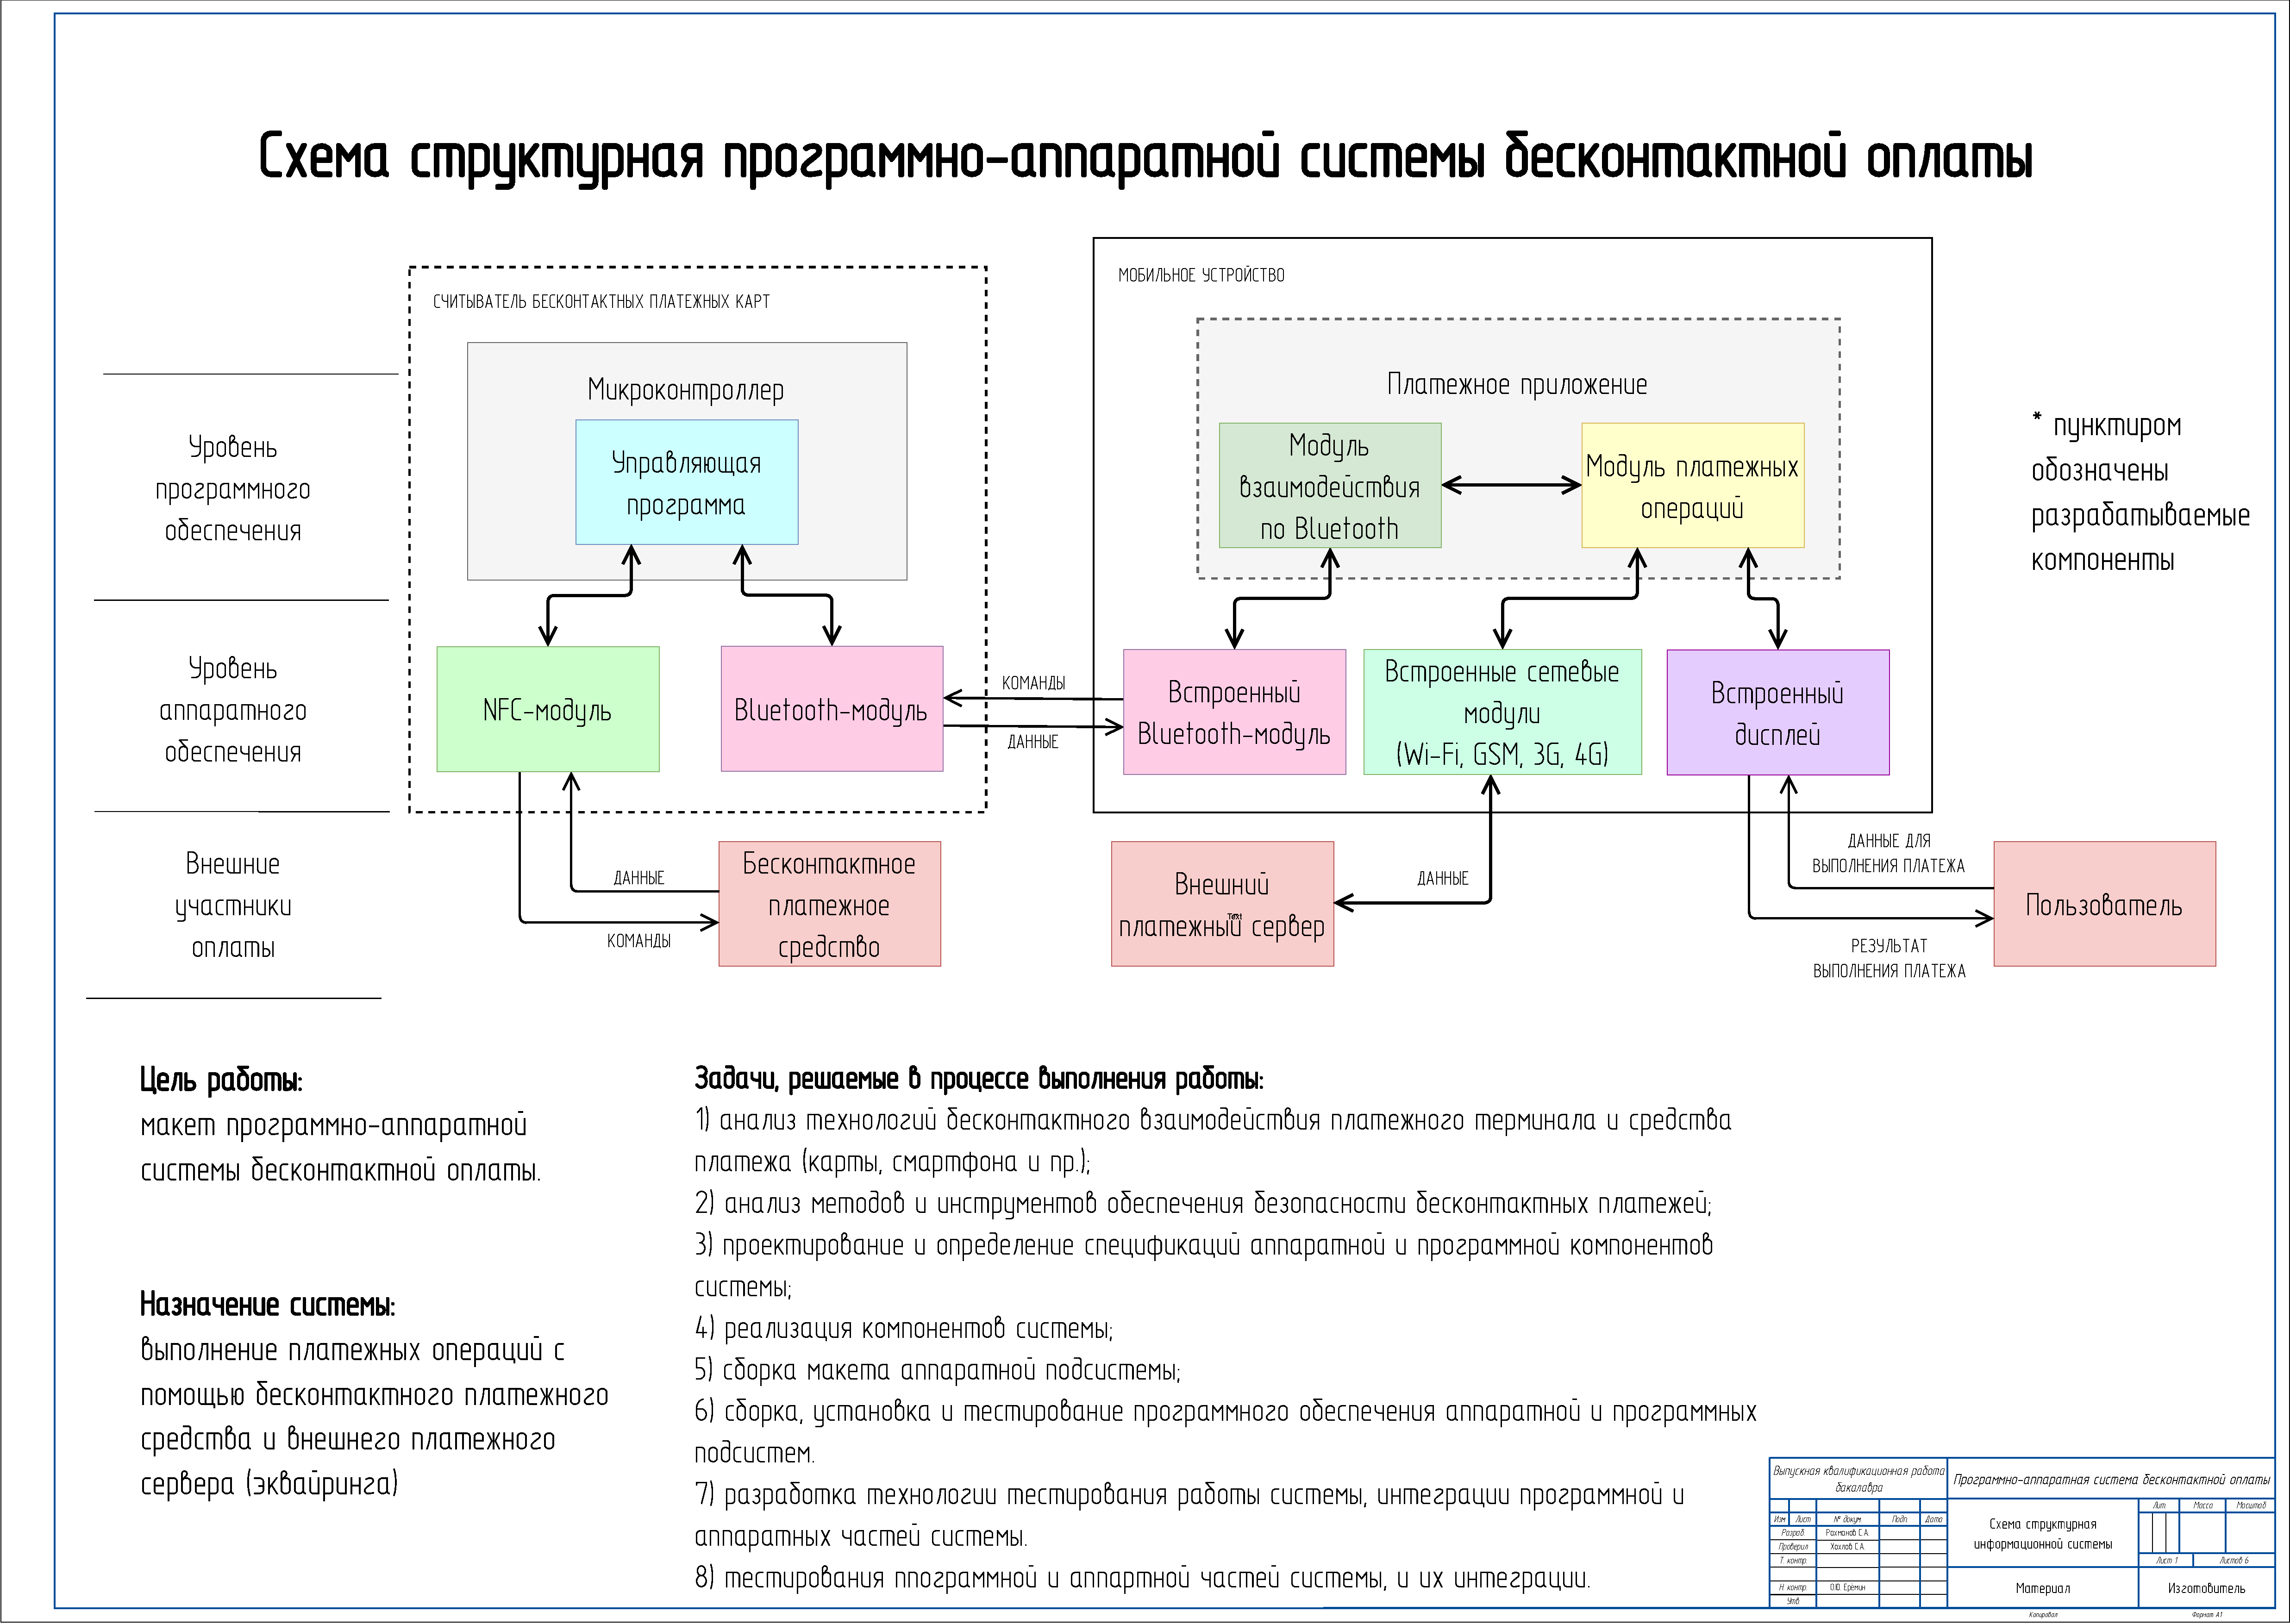
\includegraphics[angle=90,height=0.9\textheight]{appendices/schemas-1.pdf}}
    \caption{Структурная схема системы}
\end{figure}

\begin{figure}[H]
    \centering
    \fbox{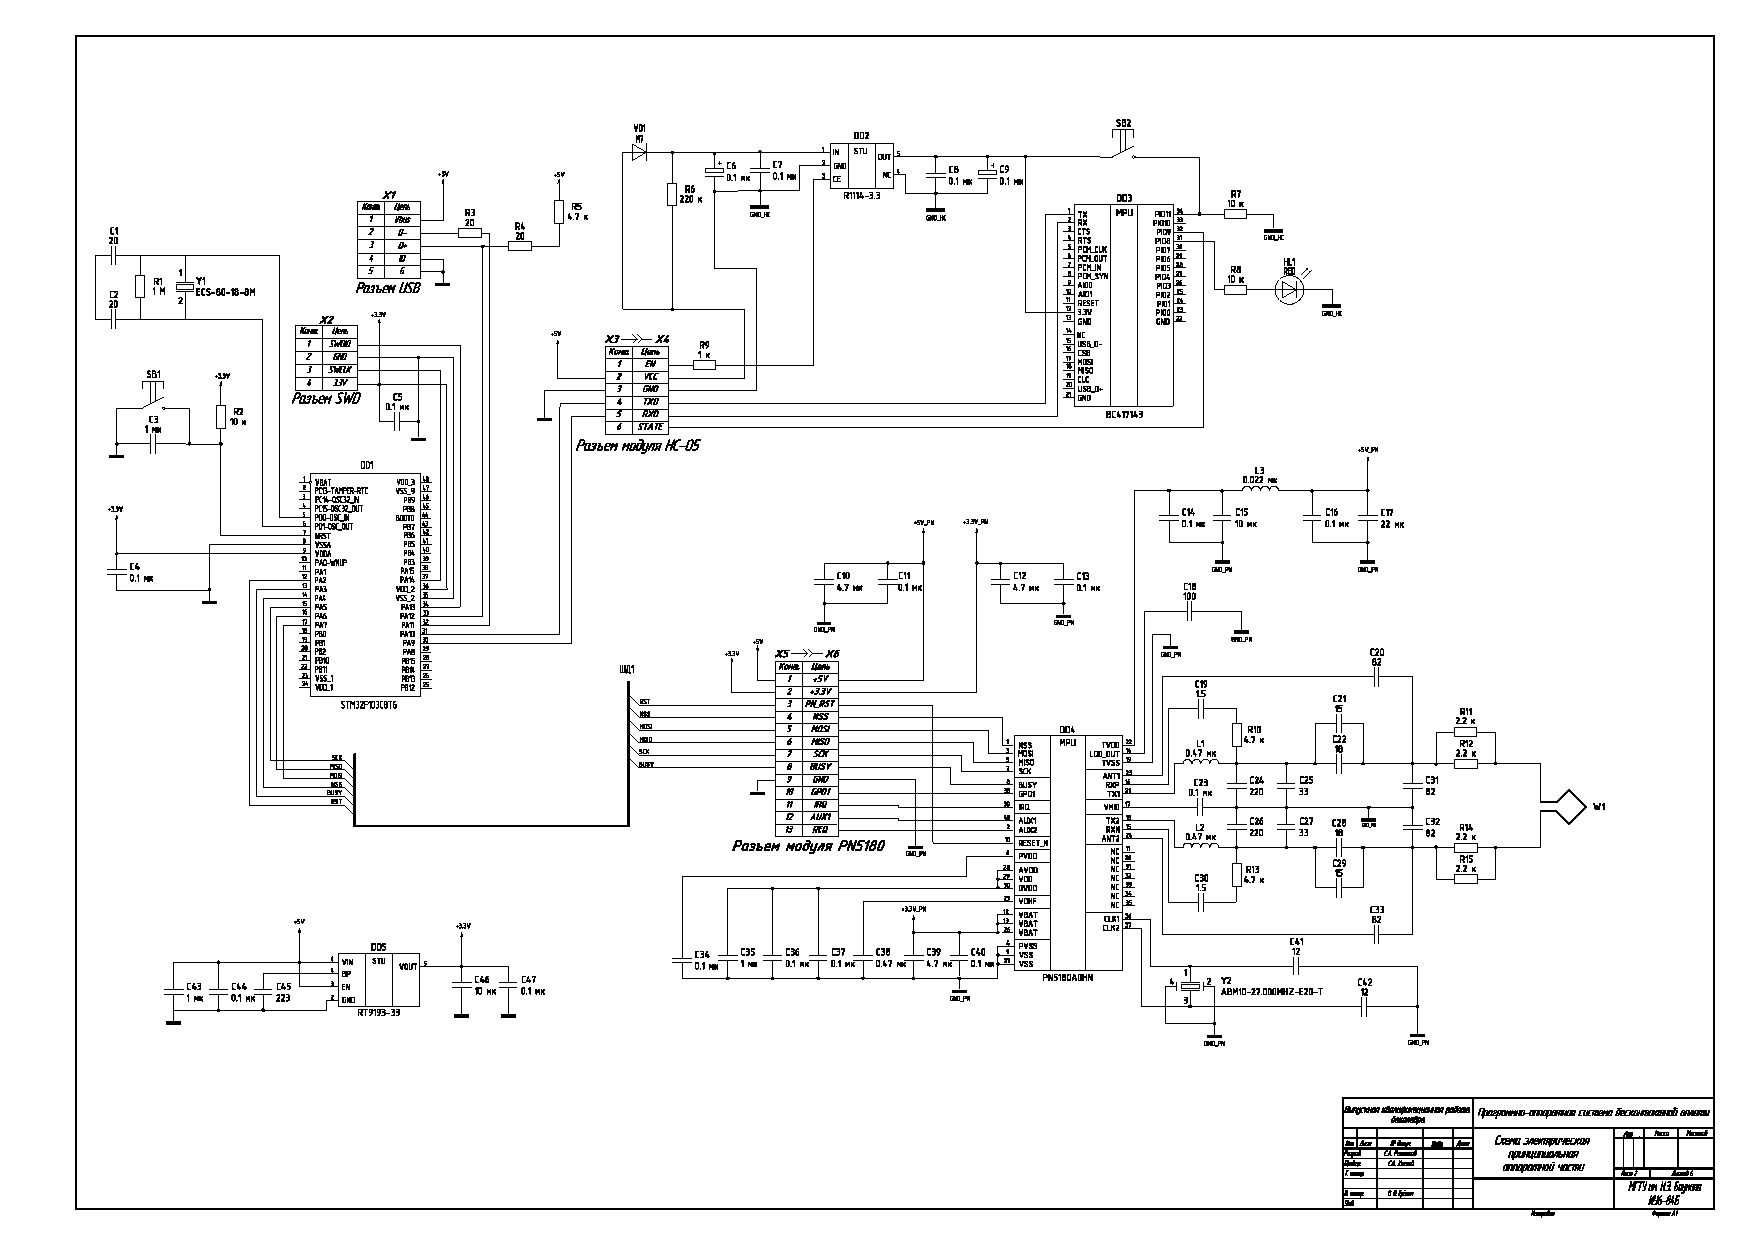
\includegraphics[angle=90,height=0.9\textheight]{appendices/schemas_princip.pdf}}
    \caption{Схема электрическая принципиальная аппаратной части системы}
\end{figure}

\begin{figure}[H]
    \centering
    \fbox{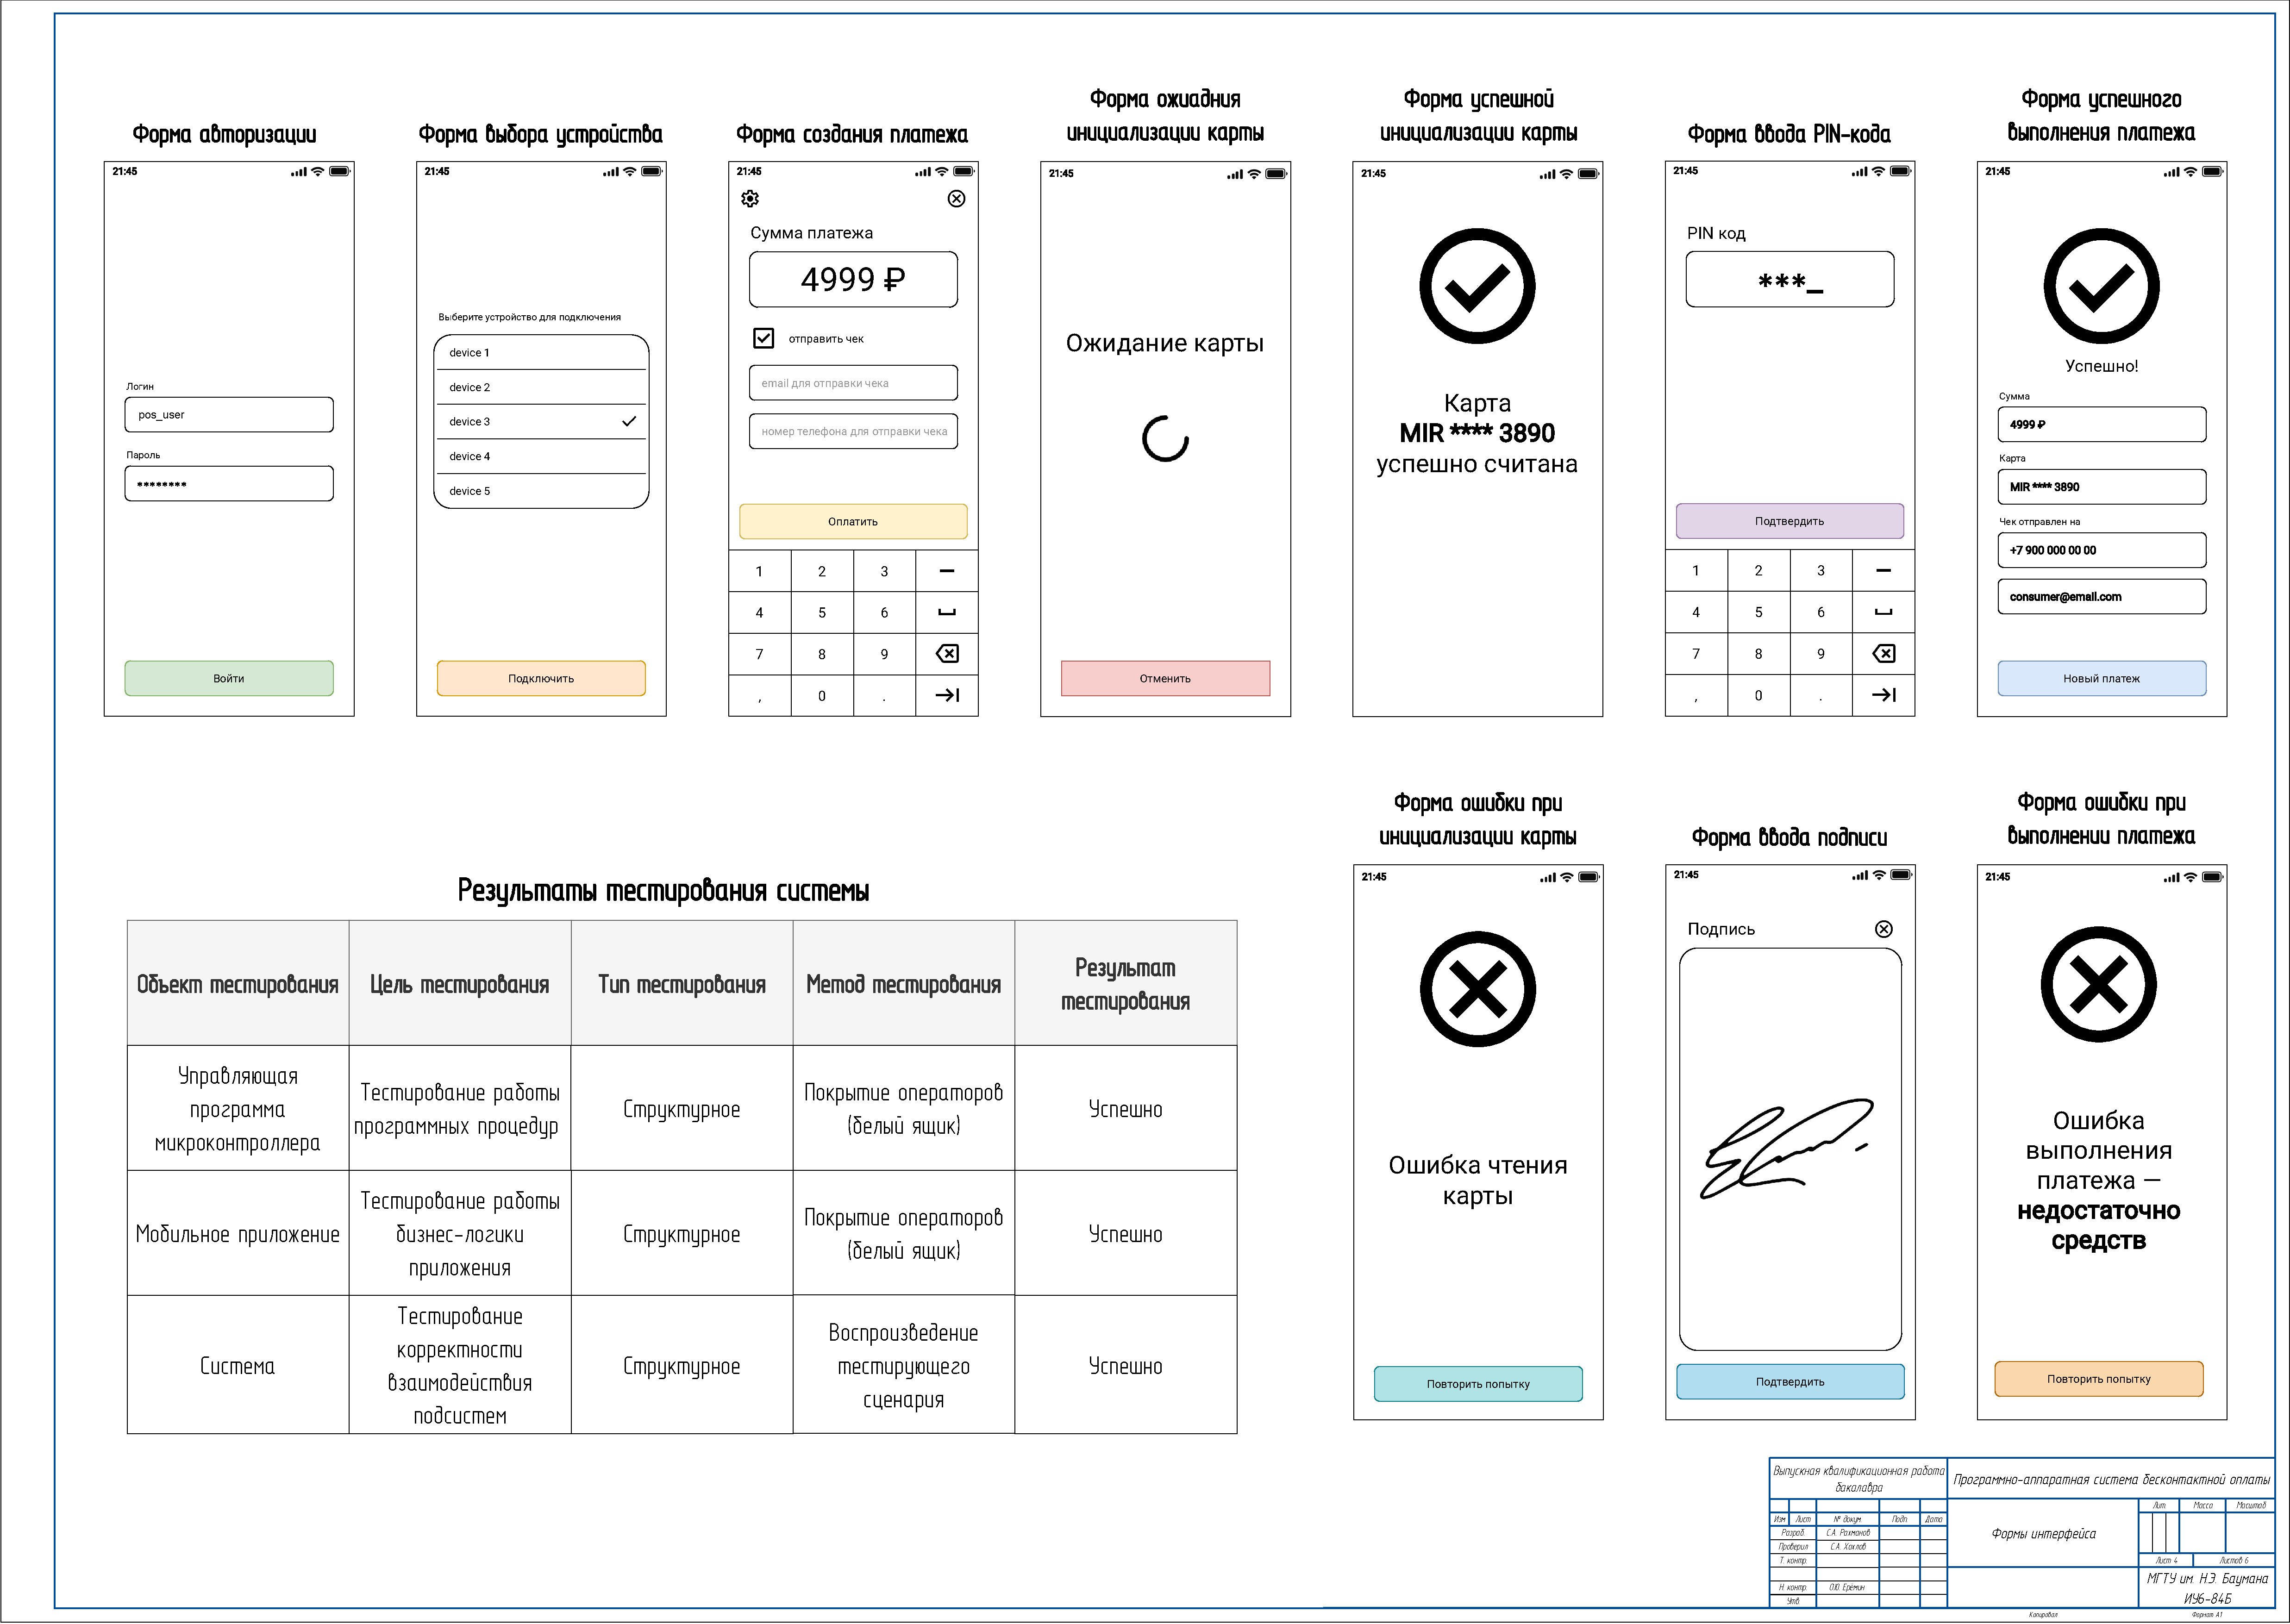
\includegraphics[angle=90,height=0.9\textheight]{appendices/schemas-3.pdf}}
    \caption{Граф состояний интерфейса}
\end{figure}

\begin{figure}[H]
    \centering
    \fbox{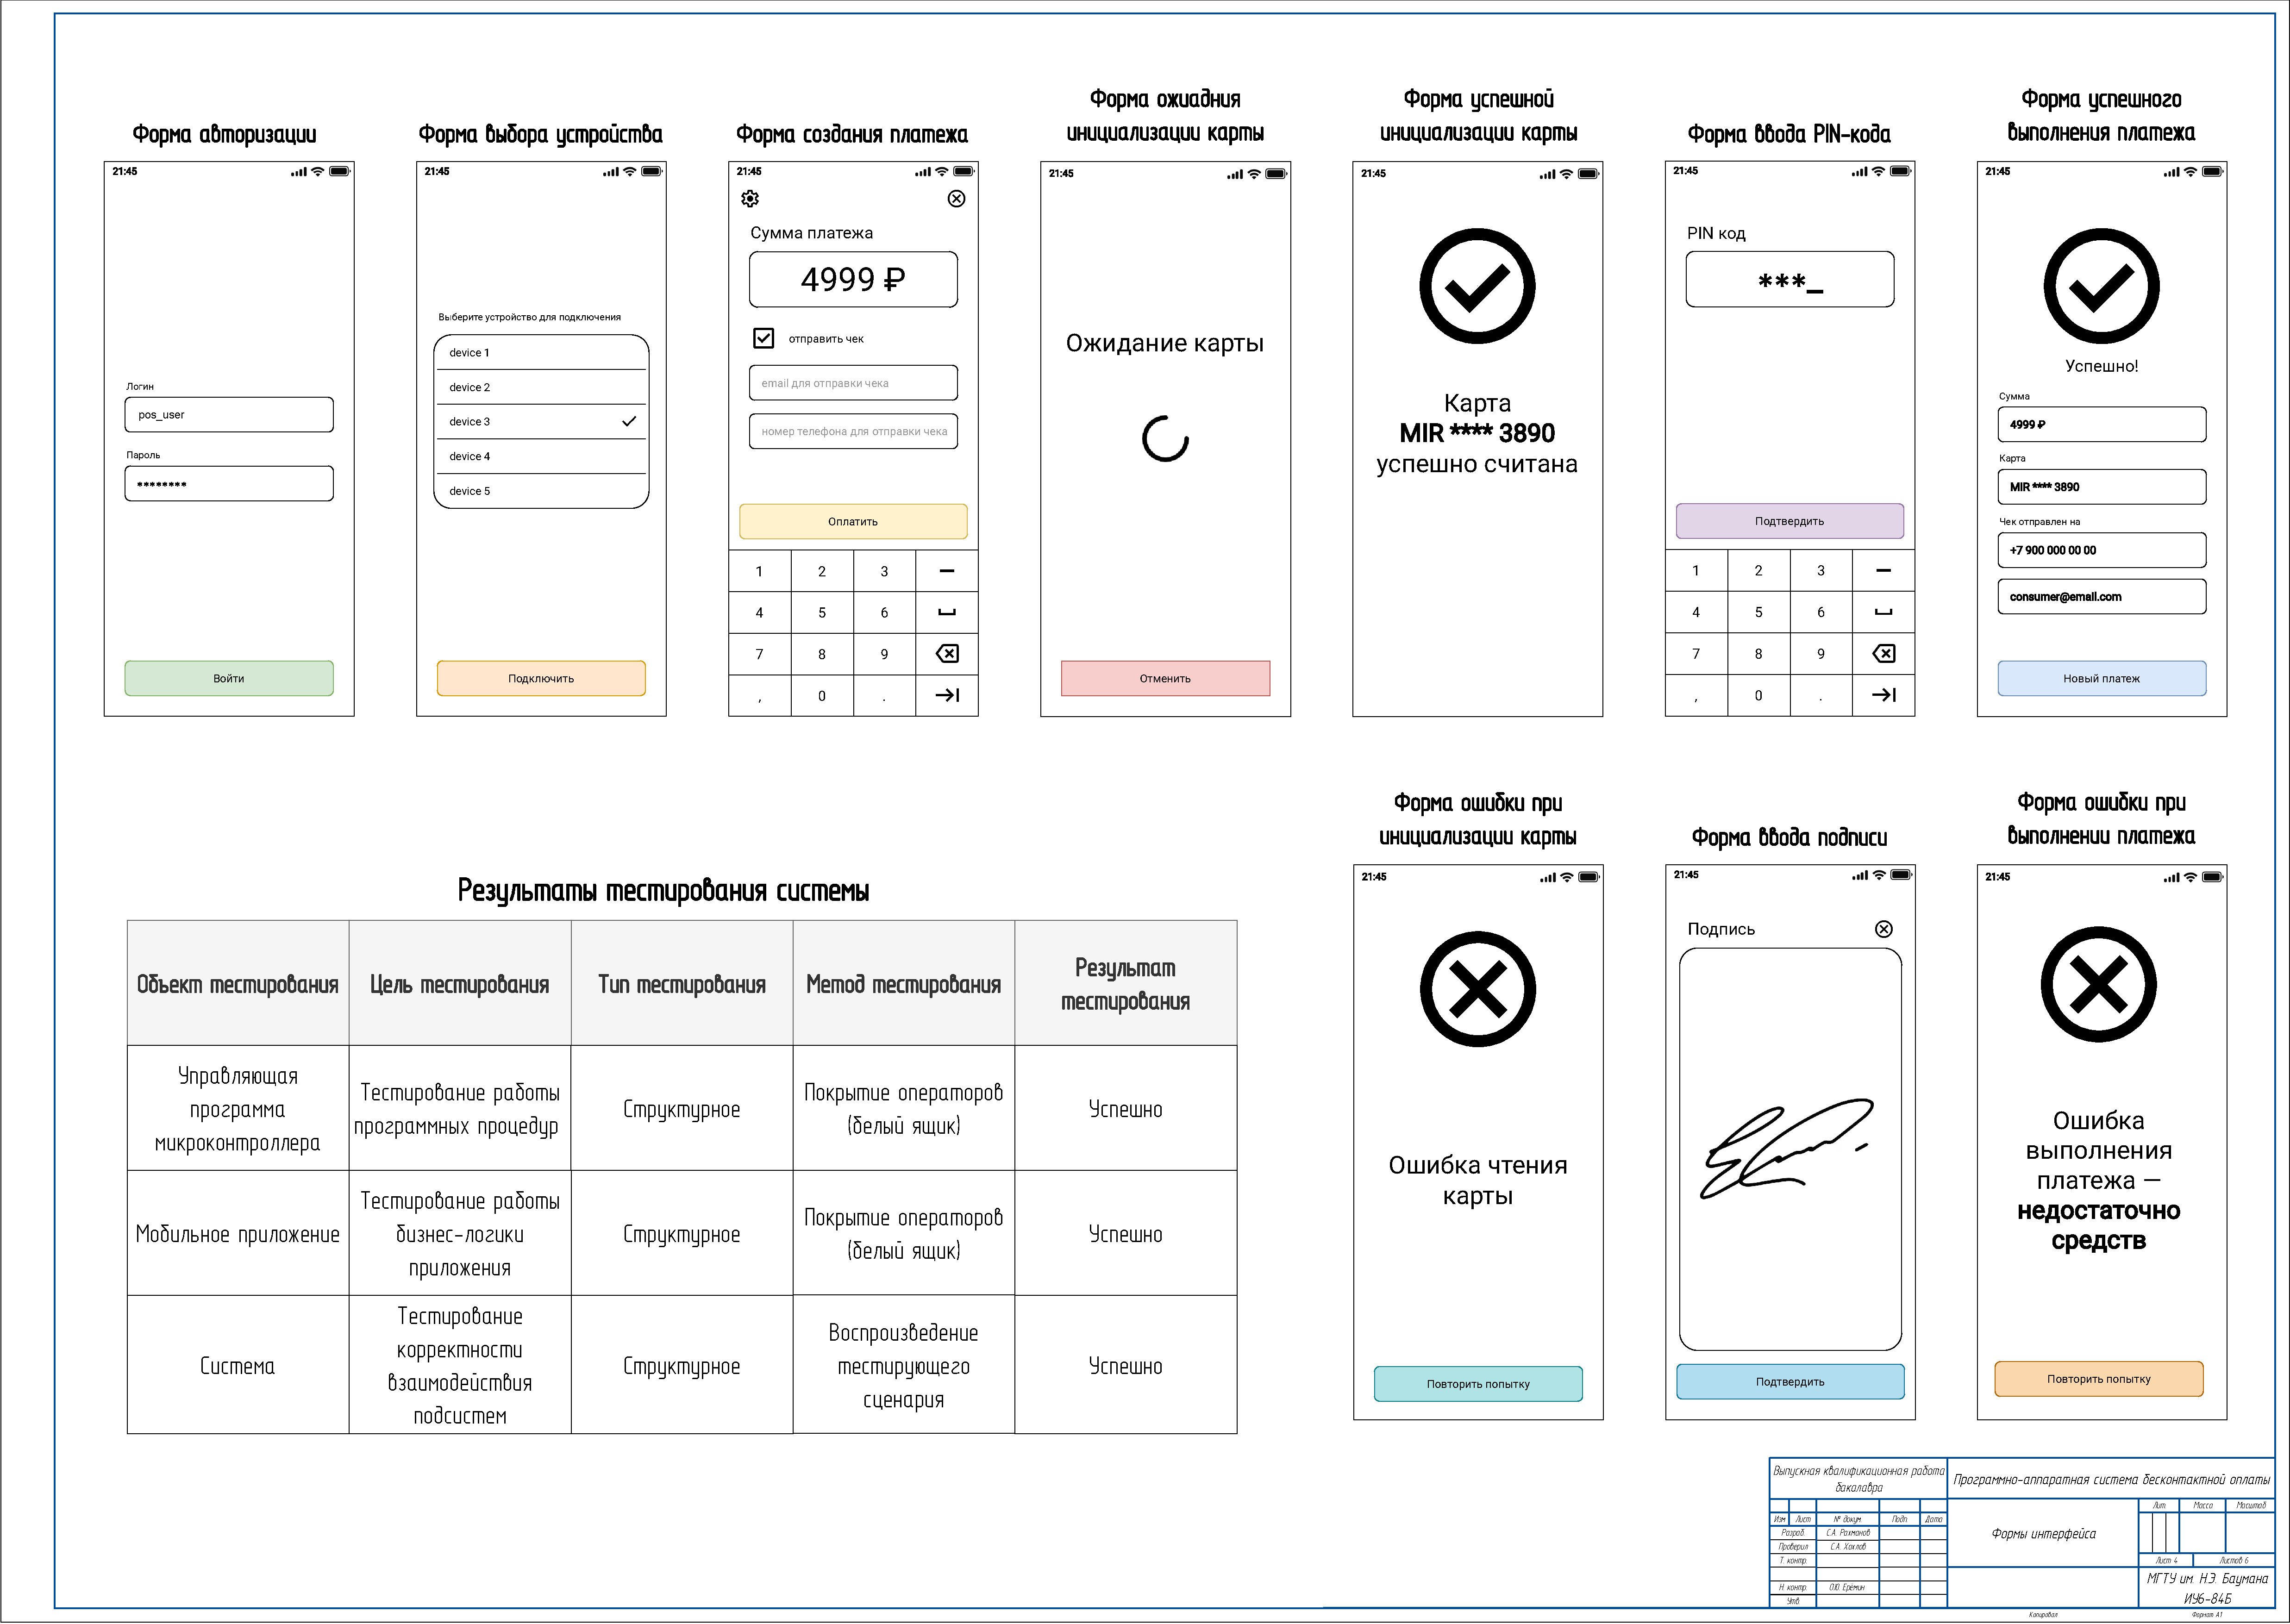
\includegraphics[angle=90,height=0.9\textheight]{appendices/schemas-4.pdf}}
    \caption{Формы интерфейса}
\end{figure}

\begin{figure}[H]
    \centering
    \fbox{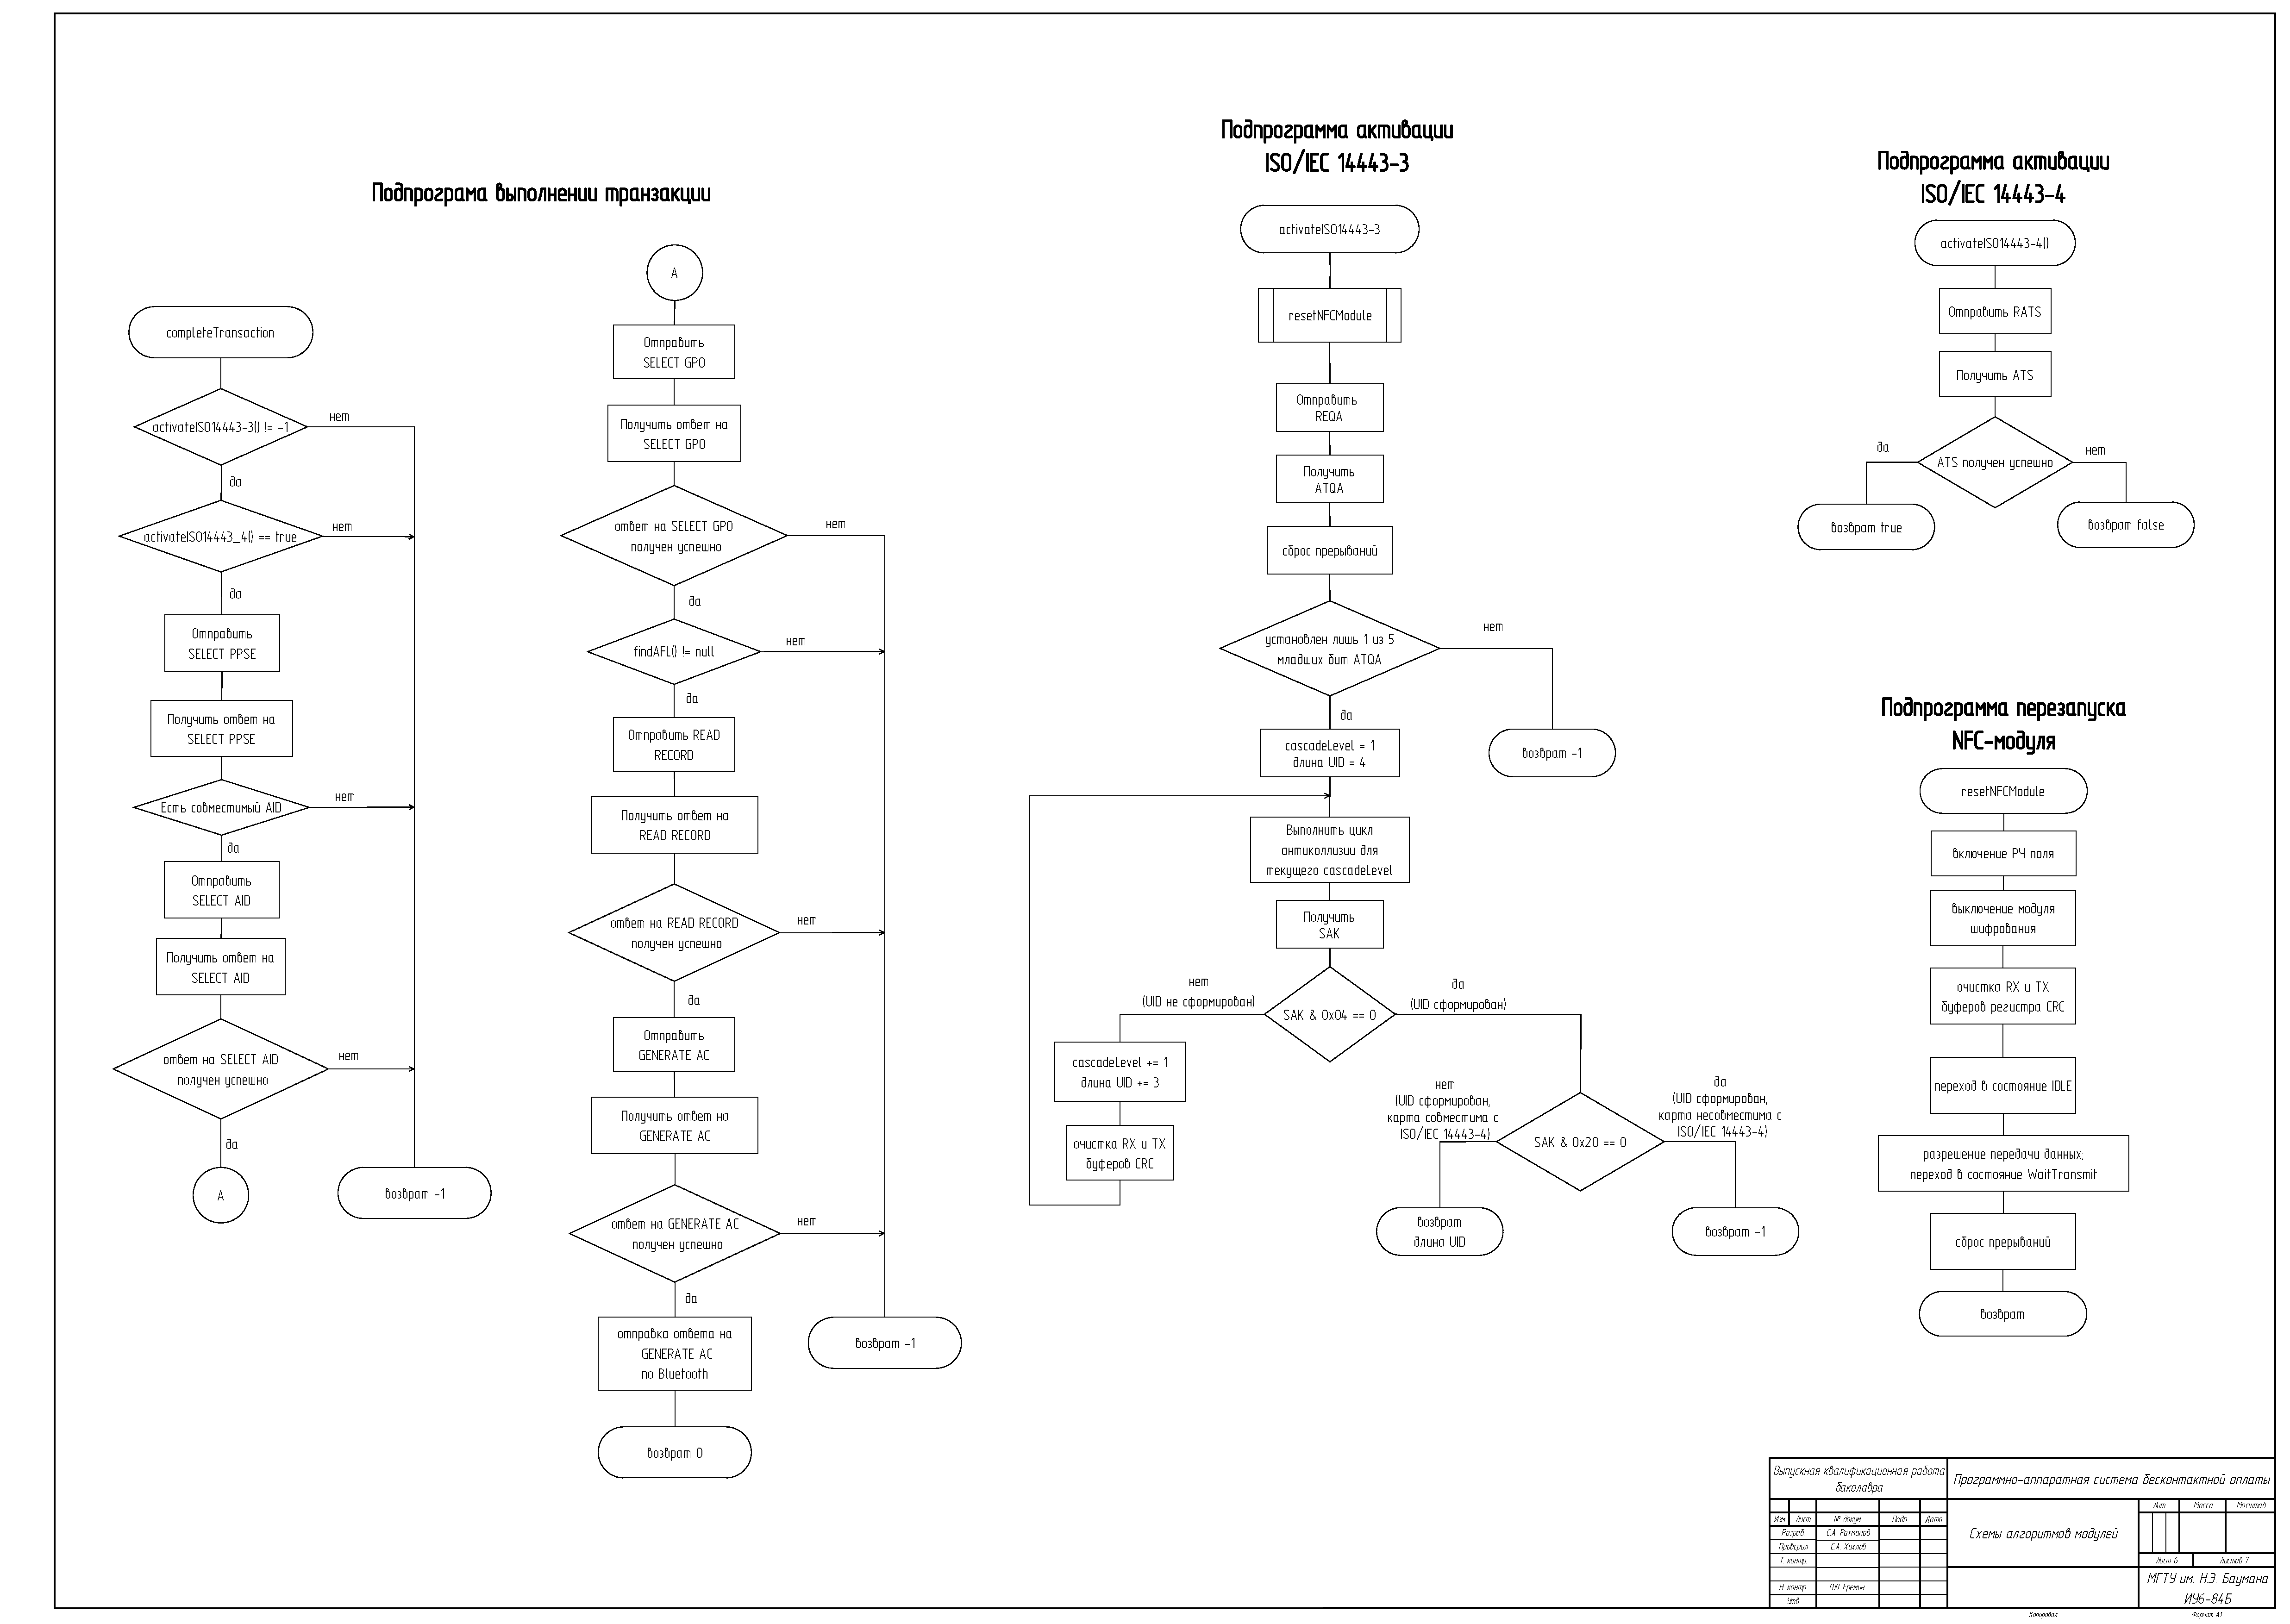
\includegraphics[angle=90,height=0.9\textheight]{appendices/schemas-5.pdf}}
    \caption{Диаграммы классов программного обеспечения}
\end{figure}

\begin{figure}[H]
    \centering
    \fbox{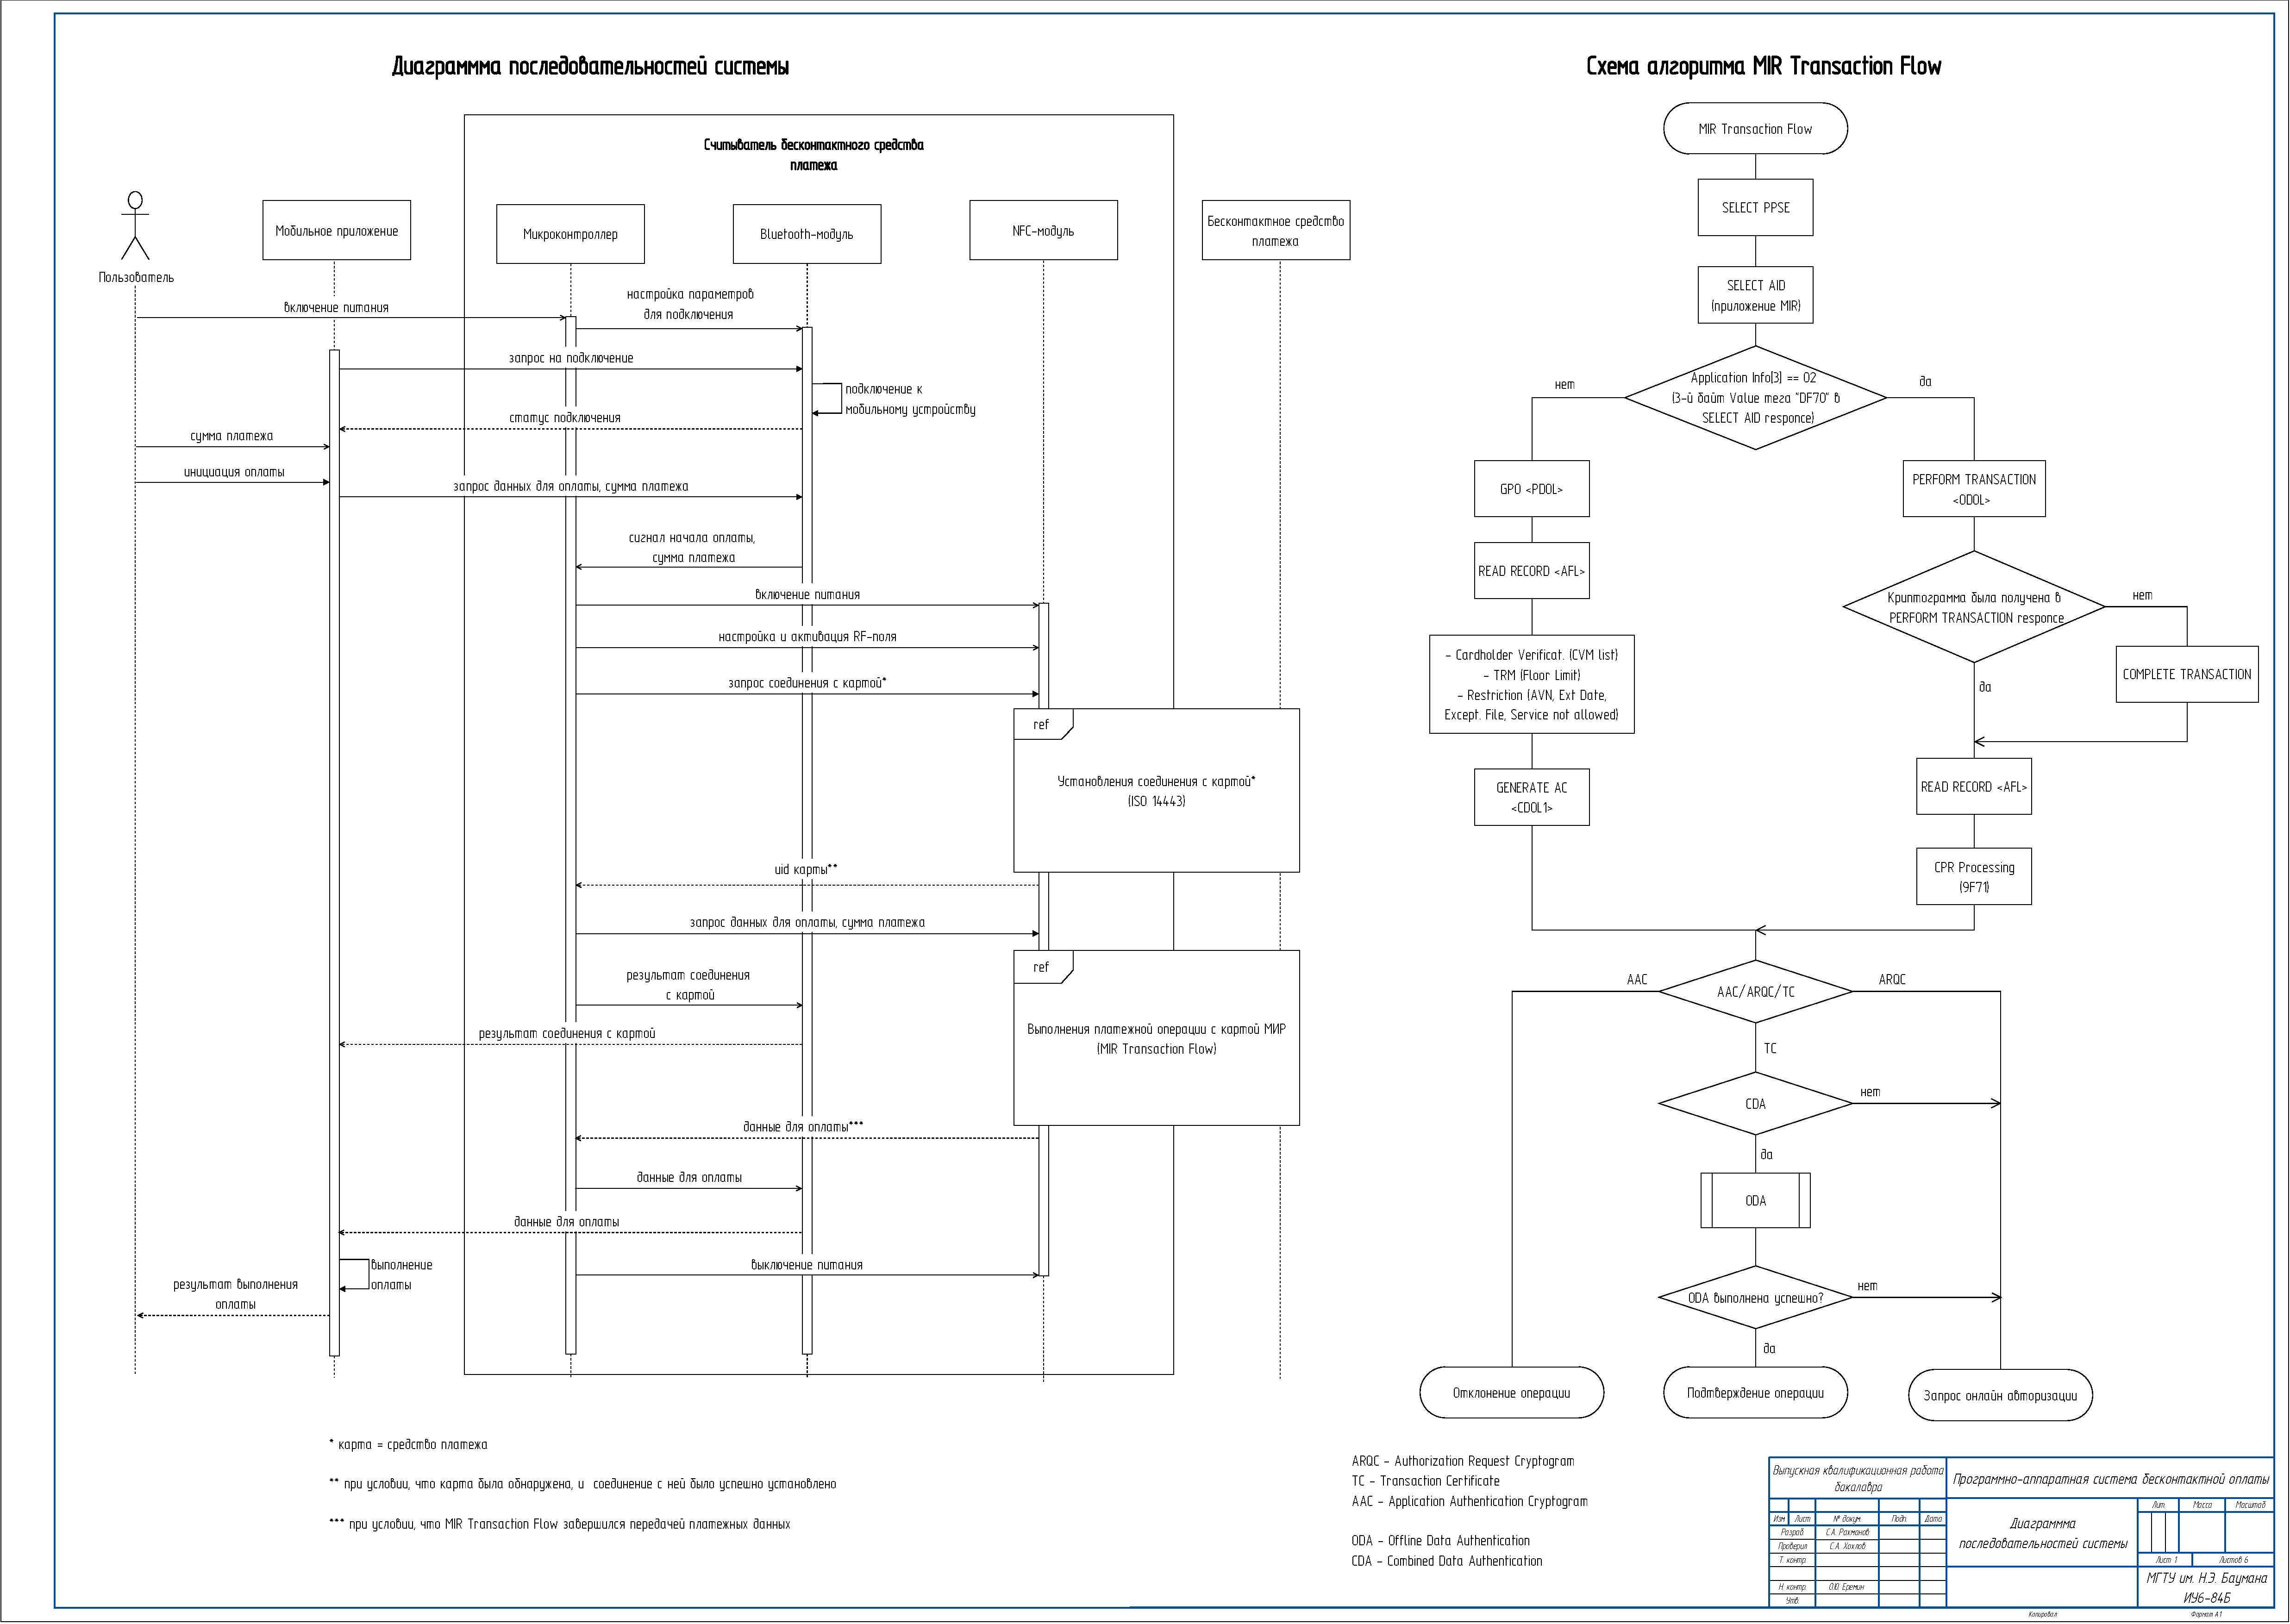
\includegraphics[angle=90,height=0.9\textheight]{appendices/schemas-6.pdf}}
    \caption{Схемы алгоритмов модулей (подпрограмм)}
\end{figure}
}
% \addtocounter{page}{6}
